\section{Introduction}
\subsection{Problem Description}
$N$ nodes are randomly placed on a 2D \textit{floorplan}. A random node within the floorplan produces a \textit{message} that should reach all users as soon as possible. Communications are slotted. Each node has a broadcast radius $R$ defined so that only the receivers within that radius from the transmitter receive the message. A node that receives more than one message in the same slot experiences a collision and isn't able to decode any of them.

After a node successfully receives a message, it keeps extracting a value from a Bernoullian RV with success probability $p$ on every slot, until it achieves success, after which it relays the message and stops.

\subsection{Performance Indexes}
The performance of a given configuration is defined through different performance indexes, namely:
\begin{itemize}
\item the time it takes a message to reach all nodes, or alternatively, the time after which every node is either stopped or waiting for a message
\item the percentage of nodes that have received the message without collisions
\item the mean percentage of nodes that experiences a collision in a given slot
\end{itemize}
\subsection{Parameters and assumptions}
The floorplan is assumed to be square and with a fixed dimension of side $L = 100$ units.

Nodes are initialized with coordinates uniformly distributed on the $x$ and $y$ axis ranging from $0$ to $L$.

For simplicity, each time slot lasts exactly $1$ second. Communication between nodes is idealized and because every message must be transmitted before the next time-slot, each transmission is assumed to last exactly $250$ ms, regardless of the actual distance between nodes.

Different simulation campaigns have the following varying parameters:
\begin{itemize}
\item $N$ number of nodes, which is an indicator of population density for a given floorplan area $[50, 100, 200, 500, 700]$
\item $R$ units of radius for each and every node. This is a constant for each node in the same simulation $[10, 30, 50, 75, 100]$ (Note that a radius of $100$ still isn't a limit case where every node is certainly connected)
\item $p$ probability of success at each time-slot for a node ready to transmit a message 

$[15\%, 30\%, 50\%, 70\%, 85\%, 100\%]$
\end{itemize}
For each combination of these parameters, we performed $33$ repetitions, in order to have statistically sound scenarios from which we could obtain reasonably meaningful and valid data.
\section{Implementation}
The following modules have been implemented:
\begin{itemize}
\item \texttt{Node} that can receive and transmit messages according to the specifications
\item \texttt{StatCollector} that retrieves statistical information from the system for each time slot, after all nodes have completed their task
\end{itemize}
For debugging purpose, a color code inside omnetpp's graphical interface has been chosen to reflect the status of each node at every instant, as can be seen in Figure \ref{fig:floorplan}

\begin{figure}
\centering
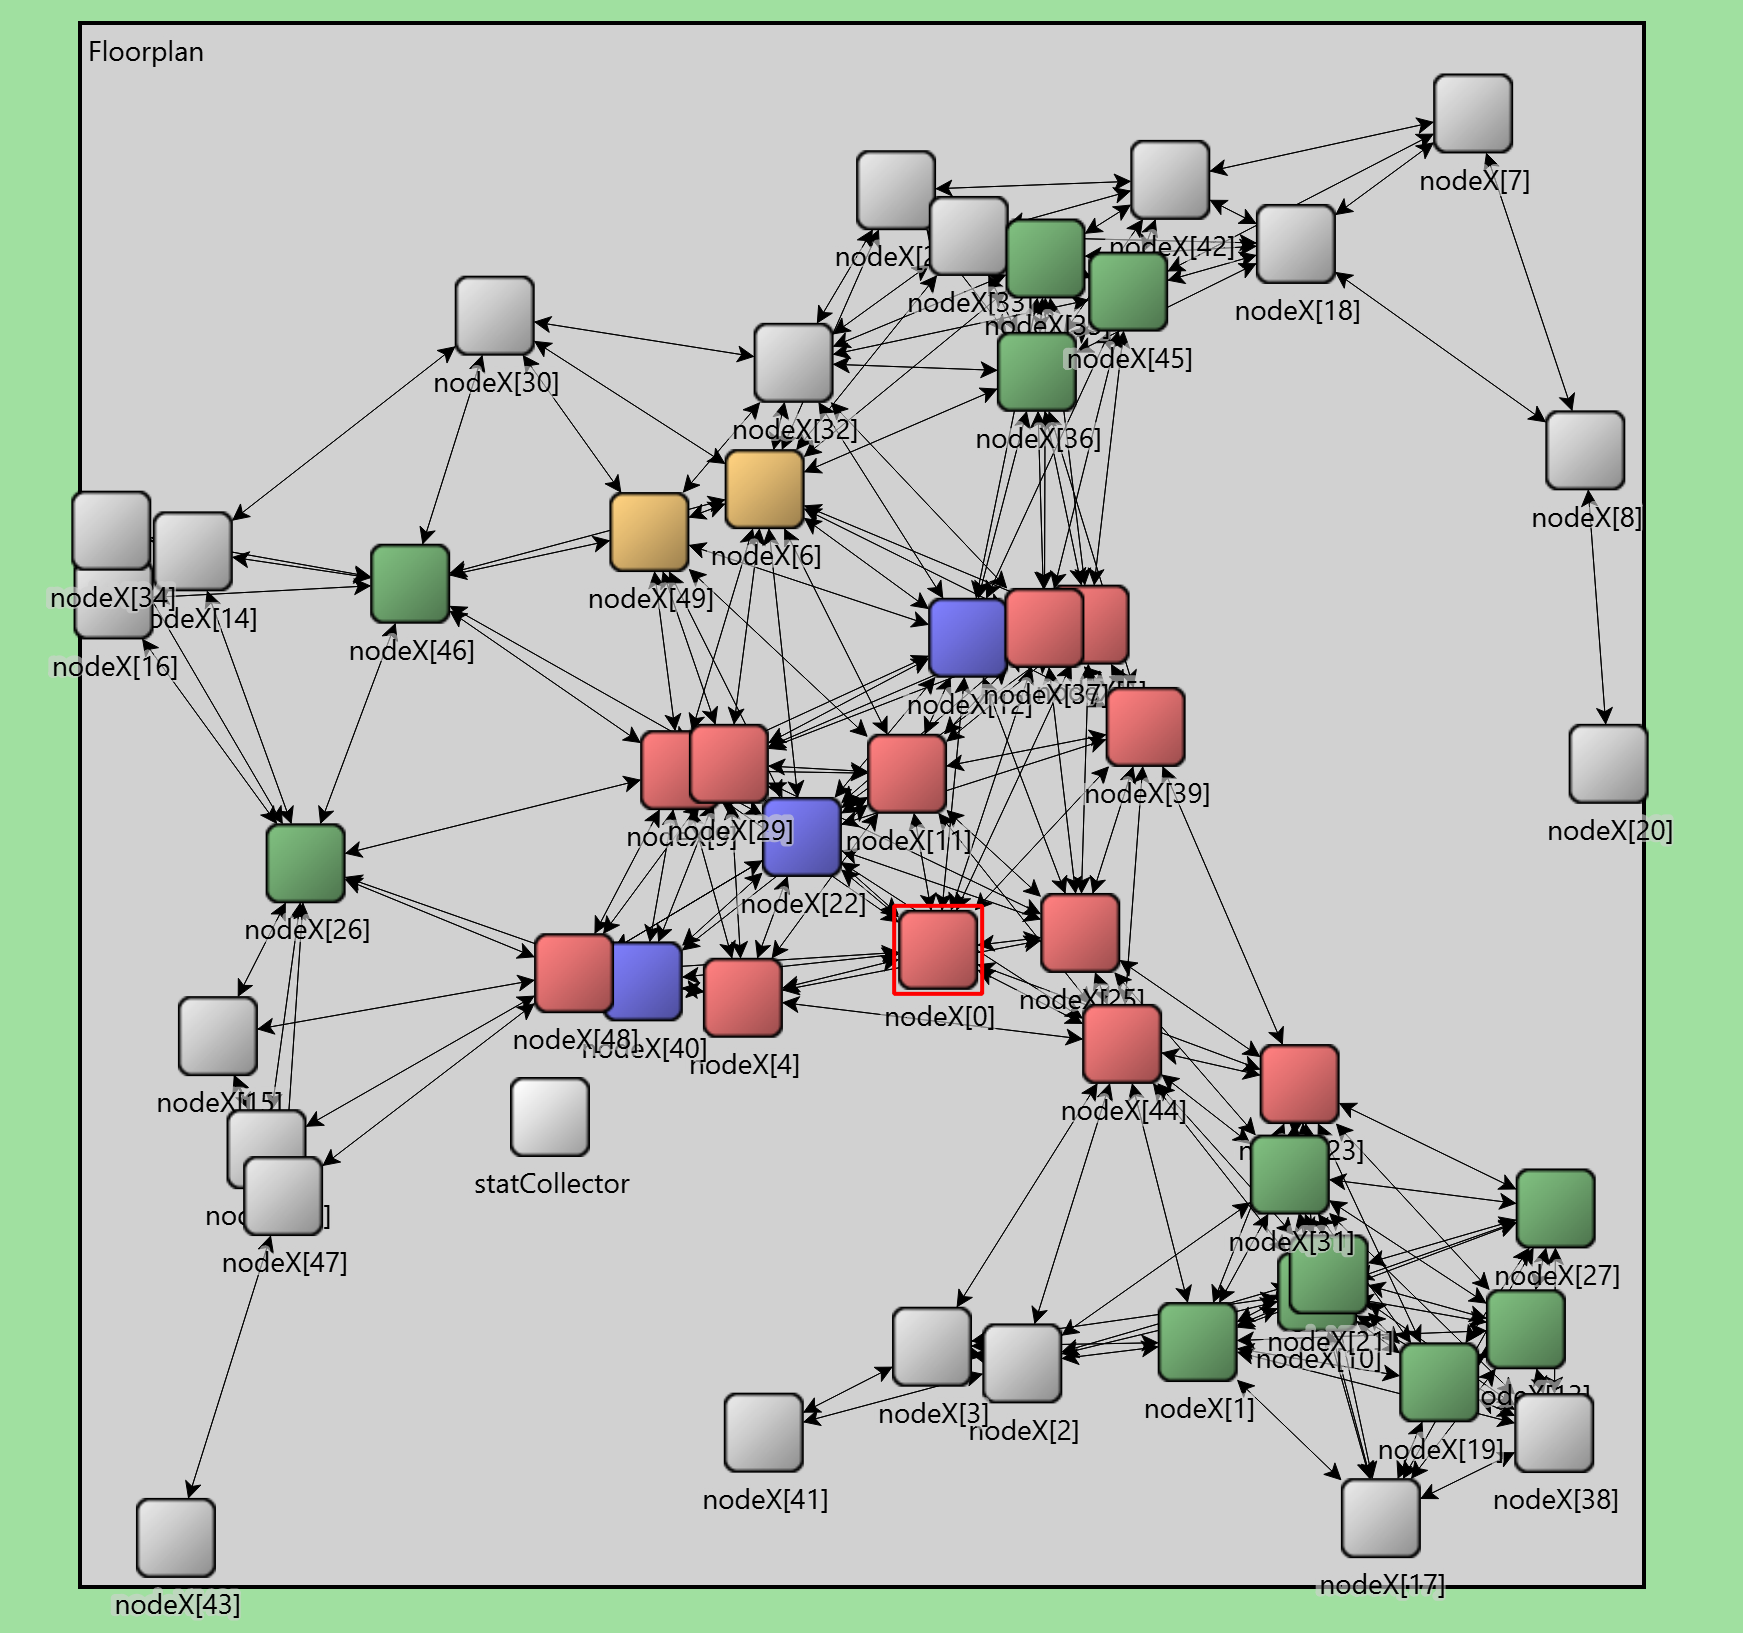
\includegraphics[width=0.8\textwidth]{./images/floorplan3.png}
\caption{debugging view of the simulated floorplan}
\label{fig:floorplan}
\end{figure}

\subsection{Node Behaviour}
A node can be found on 5 different statuses
\begin{itemize}
\item \textit{Waiting}. Node is listening for an upcoming message from one of its neighbors (gray)
\item \textit{OneMessage}. Node received exactly one message in this time slot. At the end of it, if it doesn't receive any other message, it will transition to the Ready state, otherwise it will be a Collision (blue)
\item \textit{Collision}. Node received more that one message in this time slot. In the next time slot it will restart its cycle from the Waiting state (orange)
\item \textit{Ready}. Node has a valid copy of the message. At the start of every time slot the Node extracts a Bernoullian RV with probability $p$. If it succeeds, it relays the message to its neighbors and transitions to the Done state, regardless of it having generated a collision or not. (green)
\item \textit{Done}. The node has completed its cycle. It won't respond to any more incoming messages (red)
\end{itemize}
Synchronization between nodes is idealized and isn't modeled. Each node starts its communication exactly at the beginning of the current time-slot.

\begin{figure}
\centering
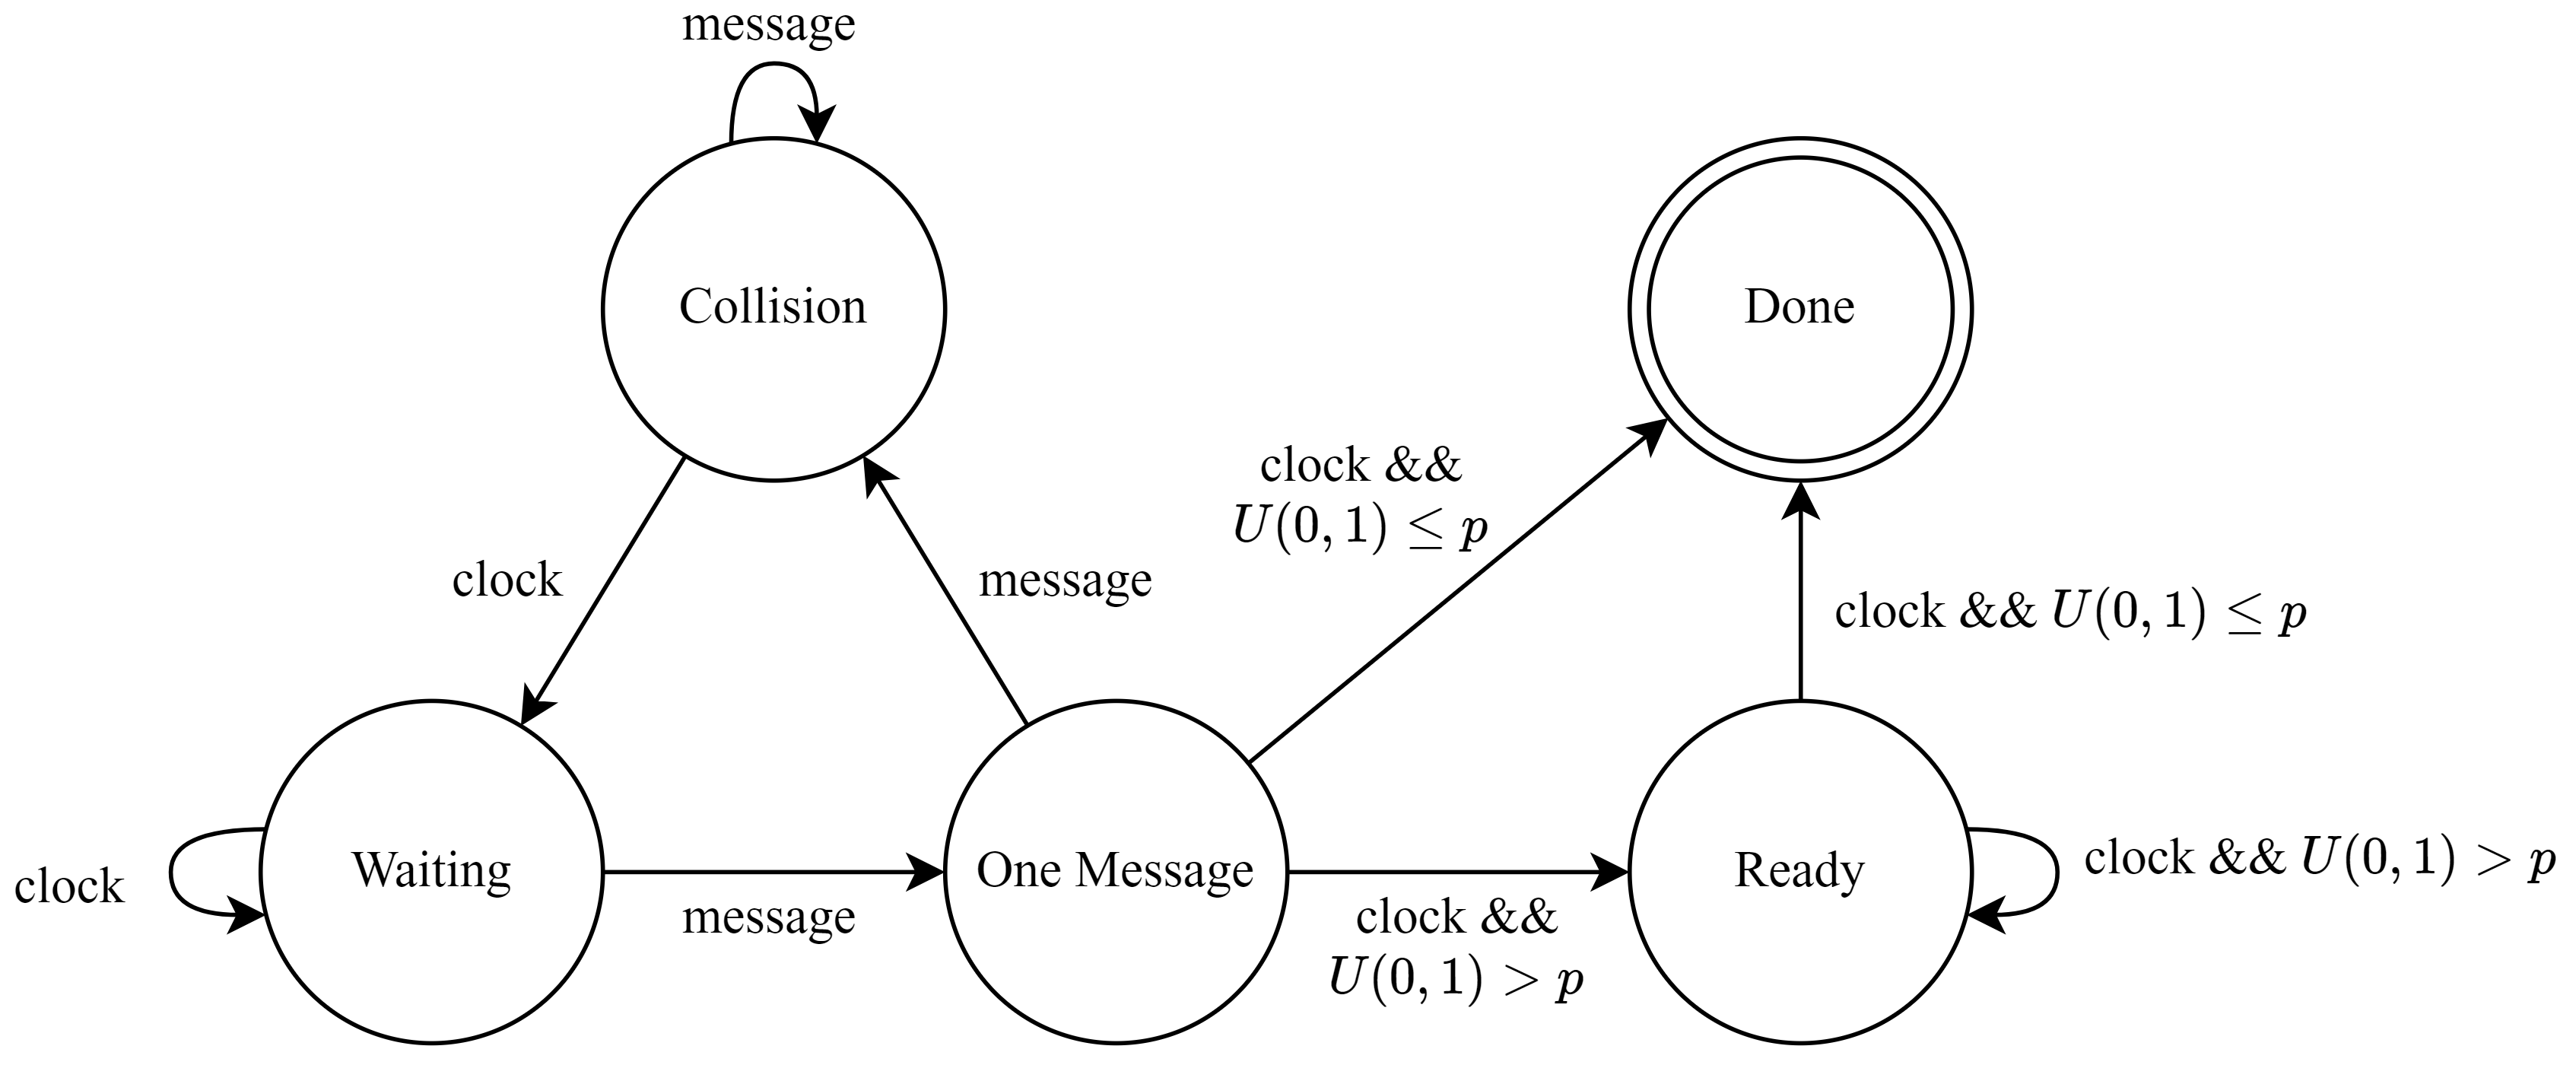
\includegraphics[width=0.8\textwidth]{./images/fsm.png}
\caption{Finite State Machine Diagram for the Node component}
\label{fig:fsm}
\end{figure}
\subsection{StatCollector Behaviour}
This module is a singleton for each simulation and isn't accessible to the rest of nodes. Because we assumed that every communication completes after $250$ ms (the delay of transmission), this modules executes with the same slotted frequency as all other nodes but with an offset of $500$ ms. This guarantees that the information retrieved by \texttt{StatCollector} comes after every node has already transitioned to the new status. From now on, if any time indication contains a $n,5$ offset, it is considered relative to the $n$-th time slot.

This module saves the relative distribution of nodes between the different statuses, i.e. what fraction of the system is in what state for each time-slot. %TODO explain it better!

\iffalse
presentazione problema
parametri analizzati
    - implementazione omnetpp
caso di studio 200Nodes (boxplot factorial-analysis model)
	tabelle scelta delle run sulla base di avg(endrate) - stdDev
approfondimento tramite boxplot dei performance indexes (endrate, endtime, collision)
analisi fattoriale su questi parametri
caso di studio specifico migliore compromesso
- spiegazione della scelta del compromesso
- fissato il punto, 2 grafici boxplot al variare di r e p
- lorenz curve for done fairness
evoluzione temporale 
- confronto tra alcune run scelte tramite grafici con media e varianza
- lorenz curve for collision repartition
- model fitting
    - verifica dei requisiti
    - analisi fattoriale
    
adesso al variare di nodes
- tabella riassuntiva dei valor medi al variare dei parametri
- approfondimento tramite boxplot di casi 50Nodes e 700Nodes
analisi fattoriale su casi specifici
	andamento influenze al variare di Nodes
confronto tra risultati di analisi fattoriali
conclusioni
- possibili espansioni su configurazione diversa del floorplan
    - densità constante, numero di nodi diverso
    - densità non costante, con modello apposito (isole con ponti)
\fi
